\author{Łukasz Ziobroń}
\title[Crisis]{(R)evolution of C++}
\institute{lukasz@ziobron.net \and \url{http://ziobron.net}}
\date{code::dive, 2016-11-15}
\subject{Computer Science}
\subtitle{aka The Hitchhiker's Guide to the C++}
%\logo{}

\begin{frame}
\titlepage
\end{frame}

\begin{frame}
  \frametitle{(R)evolution of JS}
  \centering 
  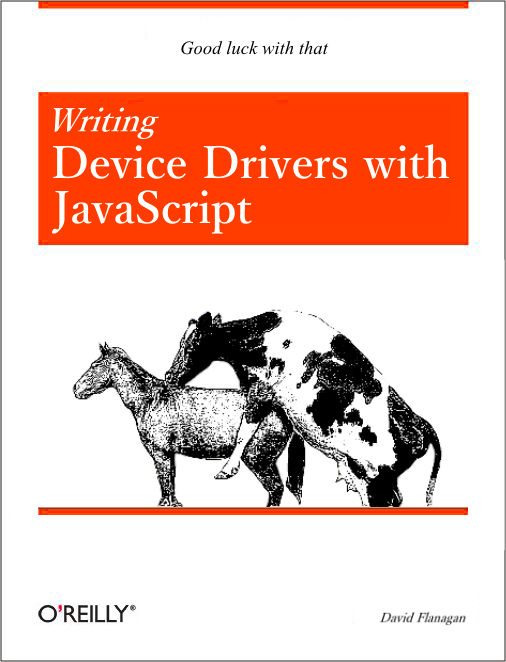
\includegraphics[height=0.8\paperheight]{writing-device-drivers-with-js}
\end{frame}

\begin{frame}
  \frametitle{About the author}
  \begin{columns}
    \column{0.3\textwidth}
      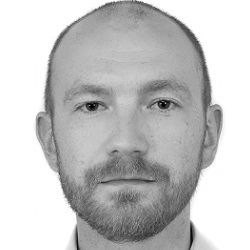
\includegraphics[height=100pt]{LukaszZiobron}
    \column{0.7\textwidth}
      \centering
      
\includegraphics[height=50pt]{html4-logo} \pause
      
\includegraphics[height=40pt]{php-logo} \pause
      
\includegraphics[height=50pt]{html5-logo}
      
\includegraphics[height=50pt]{css3-logo} \\ \pause
      
\includegraphics[height=50pt]{c-logo} \pause
      
\includegraphics[height=60pt]{matlab-logo} \\ \pause
      
\includegraphics[height=80pt]{c++-logo} \pause %TODO: Wyszarzyć wszystko poza c++
      
\includegraphics[height=65pt]{python-logo}
  \end{columns}
\end{frame}


\begin{frame}
    \frametitle{About the author}
    \begin{columns}
        \column{0.6\textwidth}
%        Codes in:
%        \begin{itemize}
%            \item C++
%            \item Python
%        \end{itemize}
%        Used to code in:
%        \begin{itemize}
%            \item HTML
%            \item PHP
%            \item Matlab
%        \end{itemize}
        Interests:
        \begin{itemize}%TODO: Different photos for each
            \item Archery
            \item Digital photography
            \item Machine learning
            \item Image processing
            \item High tech
            \item Blogging at \url{ziobron.net}
        \end{itemize}
        \column{0.4\textwidth}
        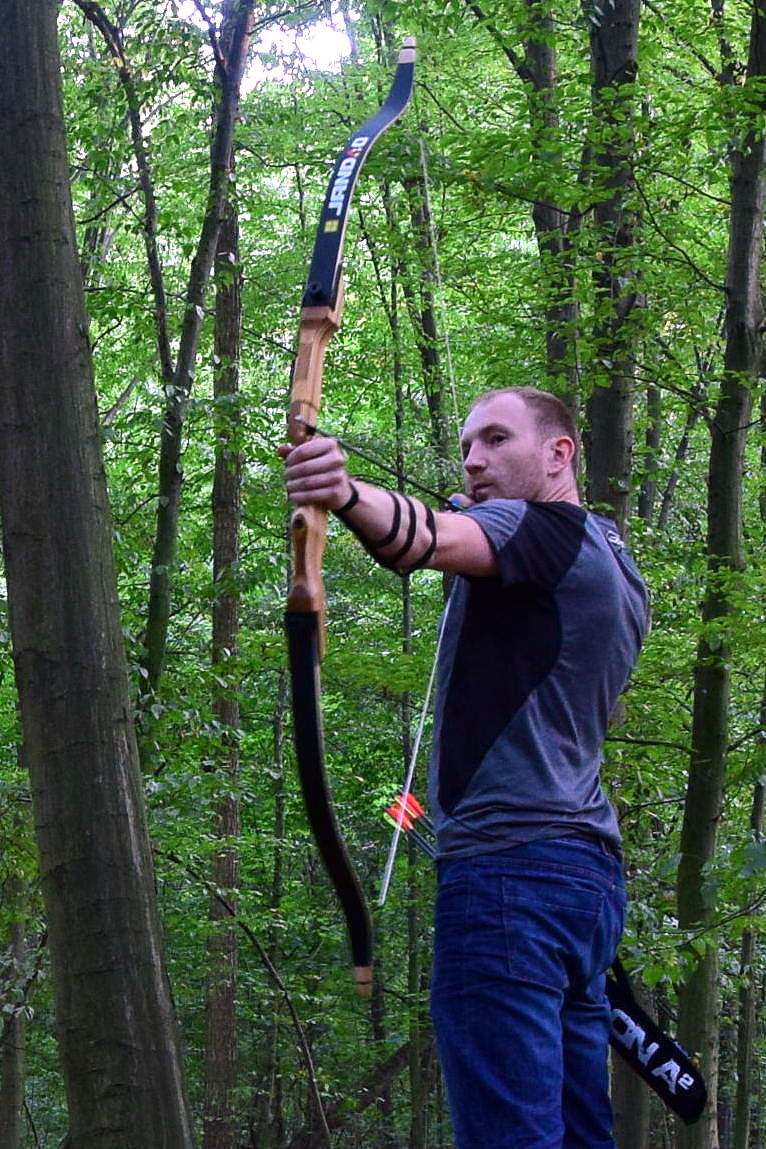
\includegraphics[height=0.75\paperheight]{archer}
%        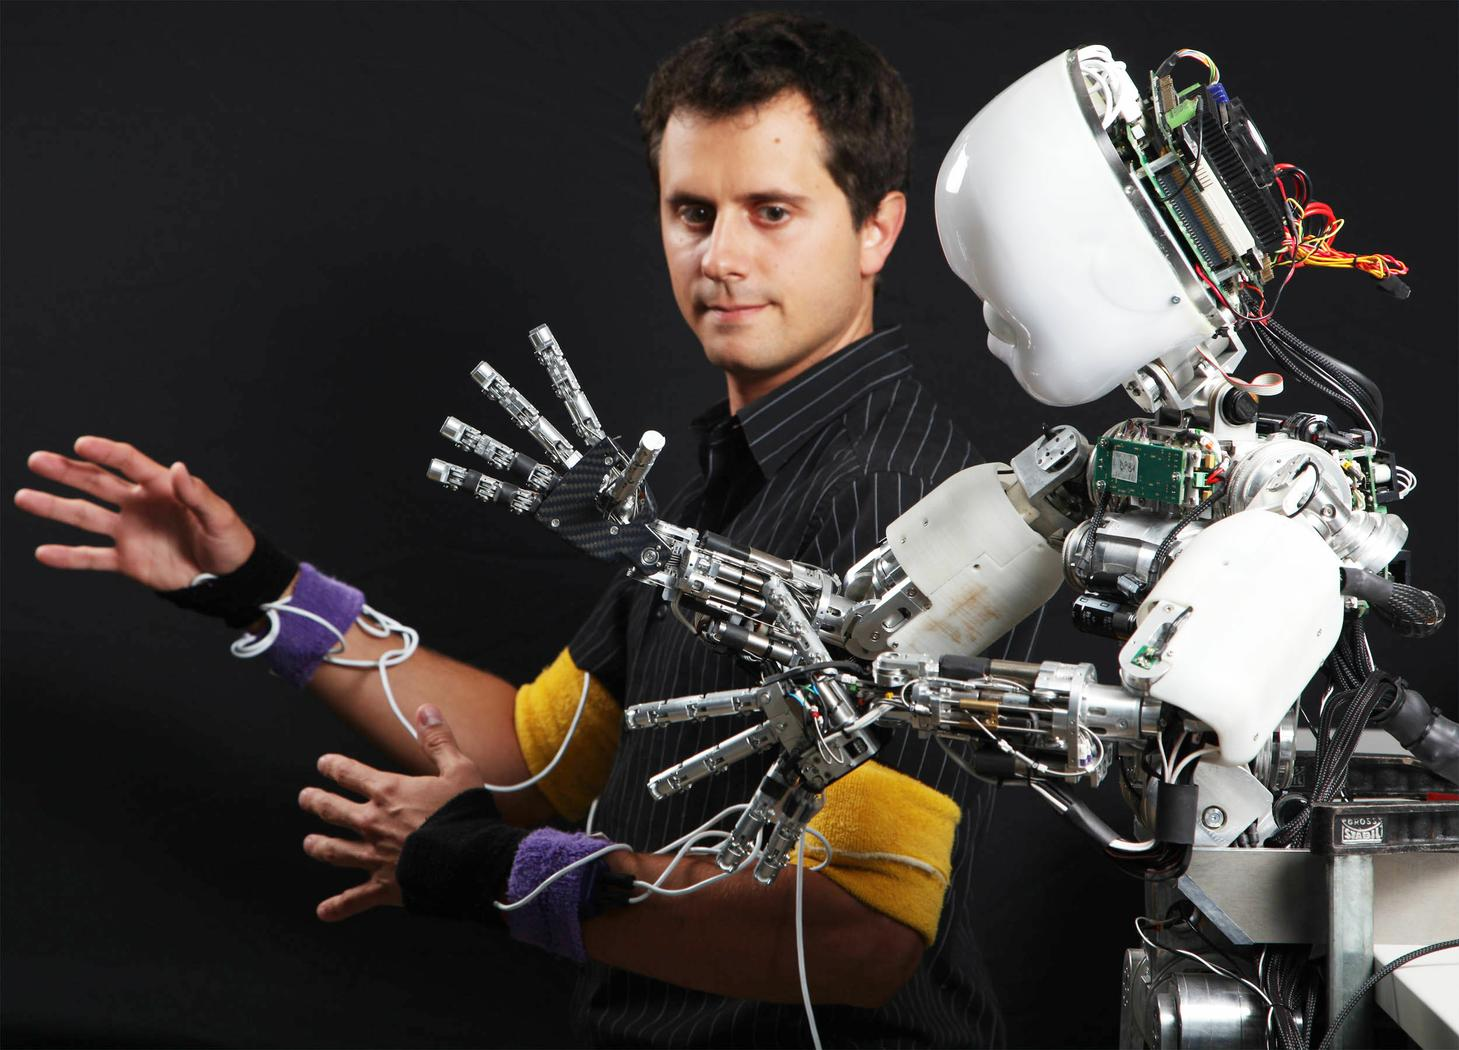
\includegraphics[height=100pt]{machine-learning-robot} \\
    \end{columns}
\end{frame}

% TODO: bold
\slide{Key messages}{
  \Large 
  \enumstep{
    \item C++ had a \textbf{clear aim}, which made it popular: to \textbf{organize code better without the loss of efficiency}
    \item C++ is even more popular now, because of new standards: \textbf{C++11} and \textbf{C++14}.
    \item C++ will be \textbf{one of the most popular programming language} in future so it's worth to invest in learning it.
  }
}

\slide{Agenda}{
  \large
  \tableofcontents
}

\sectionSlide{C with Classes}{young-bjarne}{0.7\paperwidth}{b}


\slide{Roots of C++}{
    \centering 
    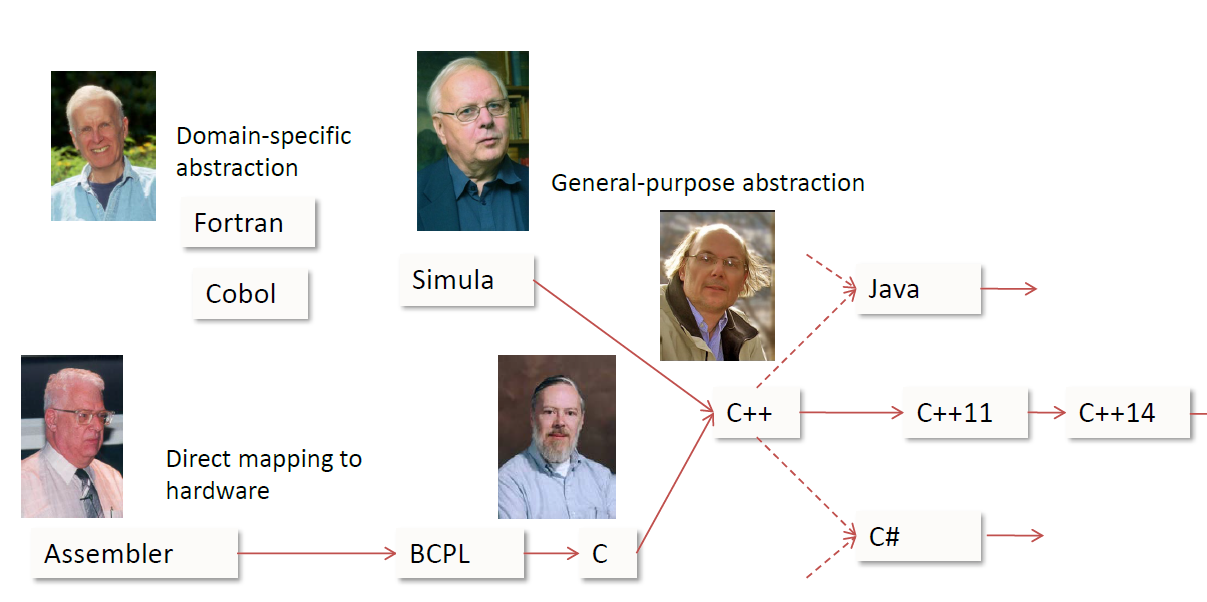
\includegraphics[height=0.8\paperheight]{cpp_roots}
    %NOTE: Before C Programming Language - Basic Combined Programming Language
}


\slide{Roots of C++}{
    Languages that were considered as a base of C++:
    \begin{itemize}
        \item Modula2
        \item Ada
        \item Smalltalk
        \item Mesa
        \item Clu
        \item C %TODO: bold, strzałka
    \end{itemize}
}


%\slide{Roots of C++}{
%    In C++ you can see the influence of 4 languages:
%    \begin{itemize}
%        \item C provided all base and syntax
%        \item Simula provided classes and inheritance
%        \item Algol68 provided:
%        \begin{itemize}
%            \item operator overloading, 
%            \item references 
%            \item ability to declare variables anywhere in a block  %NOTE: in C you had to declare variables first
%        \end{itemize}
%        \item BCPL provided // comments (later in 1985).
%    \end{itemize}
%}


\timeSlide{C with Classes}{
    Additions to C language:
    \itemstep{
        \item classes
        \item derived classes
        \item public and private access control
        \item constructors and destructors
        \item \textbf<8->{call and return functions (removed later)}
        \item friend classes
        \item type checking and conversion of function arguments
    }
}{          
    \draw[thin,blue]
    (0.5, 0) node(l1979)[anchor=west,fill=green!20,rounded corners] {\textbf{1979} C with Classes};
    
    \draw[] (1979) -- (l1979);
}

\slide{Example code in C with Classes}{
    \only<1>{\lstinputlisting{"src/c-with-classes.hpp"}}
    \only<2>{\highlightedListing{6}{6}{"src/c-with-classes.hpp"}}
    \only<3>{\highlightedListing{11}{11}{"src/c-with-classes.hpp"}}
    \only<4>{\highlightedListing{16}{18}{"src/c-with-classes.hpp"}}
}


\timeSlide{C with Classes}{
    New features added in 1981:
    \itemstep{
        \item inline functions
        \item default arguments
        \item overloading of the assignment operator
    }
}{          
    \draw[thin,blue]
    (0.5, 0) node(l1979)[anchor=west] {1979 C with Classes}
    (0.5,-0.4) node(l1981)[anchor=west,fill=green!20,rounded corners] {\textbf{1981} New features};
    
    \draw[]
    (1979) -- (l1979)
    (1981) -- (l1981);
}


\timeSlide{First standard library}{
    First elements in std lib:
    \itemstep{
        \item complex numbers
        \item string
        \item later: iostreams
    }
}{          
    \draw[thin,blue]
        (0.5, 0) node(l1979)[anchor=west] {1979 C with Classes}
        (0.5,-0.4) node(l1981)[anchor=west] {1981 New features}
        (0.5,-0.8) node(l1983)[anchor=west,fill=green!20,rounded corners] {\textbf{1983} 1st std lib};
            
    \draw[]
    (1979) -- (l1979)
    (1981) -- (l1981)
    (1983) -- (l1983);
}


\slide{C with Classes - summary}{
    \itemstep{
        \item Years of development: 1979-1983
        \item The idea was great
        \item The aim was clear:
            \begin{itemize}
                \item help programmers to organize code with classes
                \item without the loss of efficiency 
                \item and without requiring from users learning something completely new
            \end{itemize}
        \item C with Classes didn't have many users :( 
        \item It wouldn't pay to support this language in the form it was
        \item C with Classes was a "medium success"
    }
    \pause
    Bjarne knew about it and drawn conclusions.
}

\sectionSlide{Cfront era}{binario}{\paperwidth}{b}


\slide{The C++ Programming language - 1st edition (1983)}{
    %NOTE: Tell that Bjarne wrote this book to show people how to code in C++. They were reluctant to write Object Oriented code. They were skeptical. How do you learn anything new in programming? I guess that you do the same thing as I do. There are 2 schools.
    \only<1>{
        \centering 
        
\includegraphics[height=0.8\paperheight]{the-cpp-programming-language}
    }
    %NOTE: First is changing things and seeing what happens. It's easy. In that way I can learn many things.
    \only<2>{
        \centering 
        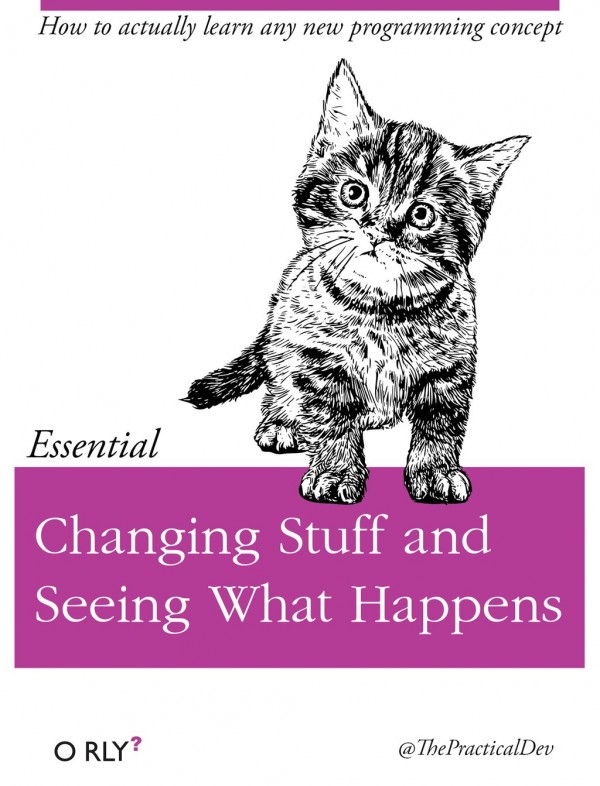
\includegraphics[height=0.8\paperheight]{changing-stuff-and-seeing-what-happens}
    }
    %NOTE: The other - just trying some stuff until it works
    \only<3>{
        \centering 
        
\includegraphics[height=0.8\paperheight]{trying-stuff-until-it-works}
    }
    %NOTE: These are really good books. I recommend them both.
    %NOTE: But the interesting fact is the opening line of that book. Bjarne put this text there:
    \begin{block}<4>{The opening line}
        \textit{``C++ is a general purpose programming language designed to make programming more enjoyable for the serious programmer''}% TODO: zostawić przekreślone
    \end{block}
    %NOTE: But reviewers weren't happy with that and couldn't believe that it was the main reason. Opening line was changed to below:
    \begin{block}<5>{The opening line}
        \textit{``C++ was designed primarily so that the author and his friends would not have to program in assembler, C, or various modern high-level languages. Its main purpose is to make writing good programs easier and more pleasant for the individual programmer''}
    \end{block}
    %NOTE: And it was accepted without any problems
}


\timeSlide{C84 and Cfront}{
    \itemstep{
        \item C with Classes got new name - C84
        \item A few months later C84 got a new name - C++
        \item First C++ compiler - Cfront
        \begin{itemize}
            \item Originally written in... C with Classes
            \item Transpiler to C code
            \item Portability matters
            \item C++ versions were named after Cfront releases
        \end{itemize}
    }
 
}{
    \draw[thin,blue]
    (0.5, 0) node(l1979)[anchor=west] {1979 C with Classes}
    (0.5,-0.4) node(l1981)[anchor=west] {1981 New features}
    (0.5,-0.7) node(l1983)[anchor=west] {1983 1st std lib}
    (0.5,-1.1) node(l1984)[anchor=west,fill=green!20,rounded corners] {\textbf{1984} C84/C++};
    
    \draw[]
    (1979) -- (l1979)
    (1981) -- (l1981)
    (1983) -- (l1983)
    (1984) -- (l1984);
}


\timeSlide{Cfront 1.0}{
    New features:
    \enumstep{
        \item Virtual functions
        \item Function name and operator overloading
        \item References
        \item Constants (const)
        \item User-controlled free-storage memory control %NOTE: New and delete operators
        \item Improved type checking
        \item Scope resolution operator (::)
        \item BCPL-style comment terminated by end-of-line
    }
    
}{
    \draw[thin,blue]
    (0.5, 0) node(l1979)[anchor=west] {1979 C with Classes}
    (0.5,-0.4) node(l1981)[anchor=west] {1981 New features}
    (0.5,-0.7) node(l1983)[anchor=west] {1983 1st std lib}
    (0.5,-1.0) node(l1984)[anchor=west] {1984 C84/C++}
    (0.5,-1.4) node(l1985)[anchor=west,fill=green!20,rounded corners] {\textbf{1985} Cfront 1.0};
    
    \draw[]
    (1979) -- (l1979)
    (1981) -- (l1981)
    (1983) -- (l1983)
    (1984) -- (l1984)
    (1985) -- (l1985);
}


\slide{Example code in C++ 1.0}{
    Virtual functions:
    \only<1>{\lstinputlisting{"src/cfront1_virtual.hpp"}}
    %NOTE: Virtual meant abstract
    \only<2>{\highlightedListing{7}{8}{"src/cfront1_virtual.hpp"}}
}


\slide{Example code in C++ 1.0}{ %TODO: zwiększyć czcionkę
    Overloaded functions:
    \only<1>{\lstinputlisting{"src/cfront1_overload.hpp"}}
%    \only<2>{\highlightedListing{1}{1}{"src/cfront1_overload.hpp"}}
}


\slide{Example code in C++ 1.0}{
    New and delete operators:
    Because you want to write that:
    \lstinputlisting[linerange={1-1}]{"src/cfront1_new.hpp"}\pause
    Instead of that:
    \lstinputlisting[linerange={3-5}]{"src/cfront1_new.hpp"}
}


\slide{Example code in C++ 1.0}{
    Improved type checking: % TODO: zaznaczyć 3 kropki na zielono
    \lstinputlisting{"src/cfront1_printf.hpp"}
}


\timeSlide{Cfront 1.1 (1986) \& Cfront 1.2 (1987)}{
    New features:
    \begin{enumerate}
        \item Bug fixes
        \item Pointers to members
        \item Protected members
    \end{enumerate}
    
}{
    \draw[thin,blue]
    (0.5, 0) node(l1979)[anchor=west] {1979 C with Classes}
    (0.5,-0.4) node(l1981)[anchor=west] {1981 New features}
    (0.5,-0.7) node(l1983)[anchor=west] {1983 1st std lib}
    (0.5,-1.0) node(l1984)[anchor=west] {1984 C84/C++}
    (0.5,-1.4) node(l1985)[anchor=west,fill=green!20,rounded corners] {\textbf{1985} Cfront 1.0};
    
    \draw[]
    (1979) -- (l1979)
    (1981) -- (l1981)
    (1983) -- (l1983)
    (1984) -- (l1984)
    (1985) -- (l1985);
}


\timeSlide{Cfront 2.0}{
    New features:
    \begin{enumerate}
        \item multiple inheritance,
        \item type-safe linkage,
        \item better resolution of overloaded functions,
        \item recursive definition of assignment and initialization,
        \item defined memory management,
        \item abstract classes,
        \item static member functions,
        \item const member functions,
        \item overloading of operator ->,
        \item protected members (first provided in release 1.2),
        \item pointers to members (first provided in release 1.2).
    \end{enumerate}
    
}{
    \draw[thin,blue]
    (0.5, 0) node(l1979)[anchor=west] {1979 C with Classes}
    (0.5,-0.4) node(l1981)[anchor=west] {1981 New features}
    (0.5,-0.7) node(l1983)[anchor=west] {1983 1st std lib}
    (0.5,-1.0) node(l1984)[anchor=west] {1984 C84/C++}
    (0.5,-1.3) node(l1985)[anchor=west] {1985 Cfront 1.0}
    (0.5,-1.7) node(l1989)[anchor=west,fill=green!20,rounded corners] {\textbf{1989} Cfront 2.0};
    
    \draw[]
    (1979) -- (l1979)
    (1981) -- (l1981)
    (1983) -- (l1983)
    (1984) -- (l1984)
    (1985) -- (l1985)
    (1989) -- (l1989);
}


\timeSlide{Cfront 3.0}{
    New features:
    \begin{enumerate}
        \item Namespaces
        \item Exceptions?
        \item Nested classes?
    \end{enumerate}
    
}{
    \draw[thin,blue]
    (0.5, 0) node(l1979)[anchor=west] {1979 C with Classes}
    (0.5,-0.4) node(l1981)[anchor=west] {1981 New features}
    (0.5,-0.7) node(l1983)[anchor=west] {1983 1st std lib}
    (0.5,-1.0) node(l1984)[anchor=west] {1984 C84/C++}
    (0.5,-1.3) node(l1985)[anchor=west] {1985 Cfront 1.0}
    (0.5,-1.6) node(l1989)[anchor=west] {1989 Cfront 2.0}
    (0.5,-2.0) node(l1991)[anchor=west,fill=green!20,rounded corners] {\textbf{1991} Cfront 3.0};
    
    \draw[]
    (1979) -- (l1979)
    (1981) -- (l1981)
    (1983) -- (l1983)
    (1984) -- (l1984)
    (1985) -- (l1985)
    (1989) -- (l1989)
    (1991) -- (l1991);
}


\timeSlide{Cfront 4.0}{
    New features:
    \begin{enumerate}
        \item Exception handling
    \end{enumerate}
    
}{
    \draw[thin,blue]
    (0.5, 0) node(l1979)[anchor=west] {1979 C with Classes}
    (0.5,-0.4) node(l1981)[anchor=west] {1981 New features}
    (0.5,-0.7) node(l1983)[anchor=west] {1983 1st std lib}
    (0.5,-1.0) node(l1984)[anchor=west] {1984 C84/C++}
    (0.5,-1.3) node(l1985)[anchor=west] {1985 Cfront 1.0}
    (0.5,-1.6) node(l1989)[anchor=west] {1989 Cfront 2.0}
    (0.5,-2.0) node(l1991)[anchor=west] {1991 Cfront 3.0}
    (0.5,-2.4) node(l1993)[anchor=west,fill=green!20,rounded corners] {\textbf{1993} Cfront 4.0};
    
    \draw[]
    (1979) -- (l1979)
    (1981) -- (l1981)
    (1983) -- (l1983)
    (1984) -- (l1984)
    (1985) -- (l1985)
    (1989) -- (l1989)
    (1991) -- (l1991)
    (1993) -- (l1993);
}





\timeSlide{Complete timeline}{
}{    
    \draw[thin,blue]
    (0.5, 0) node(l1979)[anchor=west,fill=green!20,rounded corners] {\textbf{1979} C with Classes}
    (0.5,-0.4) node(l1981)[anchor=west] {1981 New features}
    (0.5,-0.7) node(l1983)[anchor=west] {1983 1st std lib}
    (0.5,-1.0) node(l1984)[anchor=west] {1984 C84/C++ }
    (0.5,-1.3) node(l1985)[anchor=west] {1985 Cfront 1.0}
    %(0.5,-2.0) node(l1986)[anchor=west] {1986 Cfront 1.1}
    %(0.5,-2.4) node(l1987)[anchor=west] {1987 Cfront 1.2}
    (0.5,-1.6) node(l1989)[anchor=west] {1989 Cfront 2.0}
    %(0.5,-3.2) node(l1990)[anchor=west] {1990 Cfront 2.1}
    (0.5,-2.0) node(l1991)[anchor=west] {1991 Cfront 3.0}
    (0.5,-2.4) node(l1993)[anchor=west] {1993 Cfront 4.0}
    (0.5,-3.2) node(l1998)[anchor=west] {1998 C++98}
    (0.5,-4.0) node(l2003)[anchor=west] {2003 C++03}
    (0.5,-5.0) node(l2011)[anchor=west] {2011 C++11}
    (0.5,-5.5) node(l2014)[anchor=west] {2014 C++14}
    (0.5,-6.0) node(l2017)[anchor=west] {2017 C++17}
    (0.5,-6.5) node(l2020)[anchor=west] {2020 C++20};
    
    \draw[]
    (1979) -- (l1979)
    (1981) -- (l1981)
    (1983) -- (l1983)
    (1984) -- (l1984)
    (1985) -- (l1985)
    %(1986) -- (l1986)
    %(1987) -- (l1987)
    (1989) -- (l1989)
    %(1990) -- (l1990)
    (1991) -- (l1991)
    (1993) -- (l1993)
    (1998) -- (l1998)
    (2003) -- (l2003)
    (2011) -- (l2011)
    (2014) -- (l2014)
    (2017) -- (l2017)
    (2020) -- (l2020);
}


%\timelineSlide{LOL}{
%    lol
%}{
%    \textbf{1979} & \textbf{C with Classes}\\
%    1981 & New features\\
%    1983 & 1st std lib\\
%    1984 & C84/C++\\
%    1985 & Cfront 1.0\\
%    1989 & Cfront 2.0\\
%    1991 & Cfront 3.0\\
%    1993 & Cfront 4.0\\
%    1998 & C++98\\
%    2003 & C++03\\
%    2011 & C++11\\
%    2014 & C++14\\
%    2017 & C++17\\
%    2020 & C++20\\
%}
\sectionSlide{Standardization time}{elephand-toilet-standardization}{0.67\paperwidth}{b}


\timeSlide{1998 - First ISO C++ standard}{
    Features:
    \itemstep{
        \item RTTI (dynamic\_cast, typeid)
        \item covariant return types
        \item cast operators
        \item mutable
        \item bool
        \item declarations in conditions
        \item template instantiations,
        \item member templates
        \item export
    }
}{    
	\draw[thin,blue]
	(0.5, 0) node(l1979)[anchor=west] {1979 C with Classes}
	(0.5,-0.4) node(l1981)[anchor=west] {1981 New features}
	(0.5,-0.7) node(l1983)[anchor=west] {1983 1st std lib}
	(0.5,-1.0) node(l1984)[anchor=west] {1984 C84/C++ }
	(0.5,-1.3) node(l1985)[anchor=west] {1985 Cfront 1.0}
	(0.5,-1.6) node(l1989)[anchor=west] {1989 Cfront 2.0}
	(0.5,-2.0) node(l1991)[anchor=west] {1991 Cfront 3.0}
	(0.5,-2.4) node(l1993)[anchor=west] {1993 Cfront 4.0}
	(0.5,-3.2) node(l1998)[anchor=west,fill=green!20,rounded corners] {\textbf{1998} C++98};
	
	\draw[]
	(1979) -- (l1979)
	(1981) -- (l1981)
	(1983) -- (l1983)
	(1984) -- (l1984)
	(1985) -- (l1985)
	(1989) -- (l1989)
	(1991) -- (l1991)
	(1993) -- (l1993)
	(1998) -- (l1998);
}


\timeSlide{1998 - First ISO C++ standard}{
    Library additions:
    \begin{itemize}
        \item containers
        \item algorithms
        \item iterators
        \item function objects (based on STL)
        \item locale
        \item bitset
        \item valarray
        \item auto\_ptr
        \item templatized string
        \item iostream
        \item complex
    \end{itemize}
}{    
    \draw[thin,blue]
    (0.5, 0) node(l1979)[anchor=west] {1979 C with Classes}
    (0.5,-0.4) node(l1981)[anchor=west] {1981 New features}
    (0.5,-0.7) node(l1983)[anchor=west] {1983 1st std lib}
    (0.5,-1.0) node(l1984)[anchor=west] {1984 C84/C++ }
    (0.5,-1.3) node(l1985)[anchor=west] {1985 Cfront 1.0}
    (0.5,-1.6) node(l1989)[anchor=west] {1989 Cfront 2.0}
    (0.5,-2.0) node(l1991)[anchor=west] {1991 Cfront 3.0}
    (0.5,-2.4) node(l1993)[anchor=west] {1993 Cfront 4.0}
    (0.5,-3.2) node(l1998)[anchor=west,fill=green!20,rounded corners] {\textbf{1998} C++98};
    
    \draw[]
    (1979) -- (l1979)
    (1981) -- (l1981)
    (1983) -- (l1983)
    (1984) -- (l1984)
    (1985) -- (l1985)
    (1989) -- (l1989)
    (1991) -- (l1991)
    (1993) -- (l1993)
    (1998) -- (l1998);
}


\timeSlide{C++03 - Bugfix release}{
    New feature:
    \begin{itemize}    
        \item value initialization
    \end{itemize}
    Fixes:
    \begin{itemize}
        \item 125 defects fixed
        \item defect 69: incontiguous std::vector
    \end{itemize}
}{    
    \draw[thin,blue]
    (0.5, 0) node(l1979)[anchor=west] {1979 C with Classes}
    (0.5,-0.4) node(l1981)[anchor=west] {1981 New features}
    (0.5,-0.7) node(l1983)[anchor=west] {1983 1st std lib}
    (0.5,-1.0) node(l1984)[anchor=west] {1984 C84/C++ }
    (0.5,-1.3) node(l1985)[anchor=west] {1985 Cfront 1.0}
    (0.5,-1.6) node(l1989)[anchor=west] {1989 Cfront 2.0}
    (0.5,-2.0) node(l1991)[anchor=west] {1991 Cfront 3.0}
    (0.5,-2.4) node(l1993)[anchor=west] {1993 Cfront 4.0}
    (0.5,-3.2) node(l1998)[anchor=west] {1998 C++98}
    (0.5,-4.0) node(l2003)[anchor=west,fill=green!20,rounded corners] {\textbf{2003} C++03};
    
    \draw[]
    (1979) -- (l1979)
    (1981) -- (l1981)
    (1983) -- (l1983)
    (1984) -- (l1984)
    (1985) -- (l1985)
    (1989) -- (l1989)
    (1991) -- (l1991)
    (1993) -- (l1993)
    (1998) -- (l1998)
    (2003) -- (l2003);
}


%\timeSlide{Technical Report 1}{
%    From Boost:
%    \begin{itemize}    
%        \item reference wrapper
%        \item smart pointers
%        \item result of
%        \item bind
%        \item type traits
%        \item random
%        \item mathematical special functions
%        \item tuple
%        \item array
%        \item unordered containers (including hash)
%        \item regular expressions
%    \end{itemize}
%}{    %TODO: Timeline zmienić
%    \draw[thin,blue]
%    (0.5, 0) node(l1979)[anchor=west] {1979 C with Classes}
%    (0.5,-0.4) node(l1981)[anchor=west] {1981 New features}
%    (0.5,-0.7) node(l1983)[anchor=west] {1983 1st std lib}
%    (0.5,-1.0) node(l1984)[anchor=west] {1984 C84/C++ }
%    (0.5,-1.3) node(l1985)[anchor=west] {1985 Cfront 1.0}
%    (0.5,-1.6) node(l1989)[anchor=west] {1989 Cfront 2.0}
%    (0.5,-2.0) node(l1991)[anchor=west] {1991 Cfront 3.0}
%    (0.5,-2.4) node(l1993)[anchor=west] {1993 Cfront 4.0}
%    (0.5,-3.2) node(l1998)[anchor=west] {1998 C++98}
%    (0.5,-4.0) node(l2003)[anchor=west,fill=green!20,rounded corners] {2003 C++03};
%    
%    \draw[]
%    (1979) -- (l1979)
%    (1981) -- (l1981)
%    (1983) -- (l1983)
%    (1984) -- (l1984)
%    (1985) -- (l1985)
%    (1989) -- (l1989)
%    (1991) -- (l1991)
%    (1993) -- (l1993)
%    (1998) -- (l1998)
%    (2003) -- (l2003);
%}


%\timeSlide{Technical Report 1}{
%    From C99:
%    \begin{itemize}    
%        \item mathematical functions from math.h that were new in C99
%        \item blank character class
%        \item floating-point environment
%        \item hexfloat I/O Manipulator
%        \item fixed-size integral types
%        \item the long long type
%        \item va\_copy
%        \item the snprintf() and vscanf() families of functions
%        \item the C99 conversion specifies for printf() and scanf() families of functions
%    \end{itemize}
%}{    %TODO: Timeline zmienić
%    \draw[thin,blue]
%    (0.5, 0) node(l1979)[anchor=west] {1979 C with Classes}
%    (0.5,-0.4) node(l1981)[anchor=west] {1981 New features}
%    (0.5,-0.7) node(l1983)[anchor=west] {1983 1st std lib}
%    (0.5,-1.0) node(l1984)[anchor=west] {1984 C84/C++ }
%    (0.5,-1.3) node(l1985)[anchor=west] {1985 Cfront 1.0}
%    (0.5,-1.6) node(l1989)[anchor=west] {1989 Cfront 2.0}
%    (0.5,-2.0) node(l1991)[anchor=west] {1991 Cfront 3.0}
%    (0.5,-2.4) node(l1993)[anchor=west] {1993 Cfront 4.0}
%    (0.5,-3.2) node(l1998)[anchor=west] {1998 C++98}
%    (0.5,-4.0) node(l2003)[anchor=west,fill=green!20,rounded corners] {2003 C++03};
%    
%    \draw[]
%    (1979) -- (l1979)
%    (1981) -- (l1981)
%    (1983) -- (l1983)
%    (1984) -- (l1984)
%    (1985) -- (l1985)
%    (1989) -- (l1989)
%    (1991) -- (l1991)
%    (1993) -- (l1993)
%    (1998) -- (l1998)
%    (2003) -- (l2003);
%}


\slide{C++0x}{
    \begin{block}{}
        \begin{quotation}
            {\large ``C++11 feels like a new language''}
        \end{quotation}
        \rightline{{\rm --- Bjarne Stroustrup}}
    \end{block}
    \pause
    \begin{block}{}
        \begin{quotation}
            \large
            C++0x == C++11 \pause (for x = 0xB)
        \end{quotation}
    \end{block}
}


\timeSlide{C++11}{
    New language features:
    \begin{itemize}    
        \item auto and decltype
        \item default, delete, final, override keywords
        \item rvalue references
        \item move constructors / move assignment
        \item scoped enums
        \item constexpr and literal types
        \item list initialization, brace initializers
        \item delegating constructors
        \item nullptr
        \item long long, char16\_t and char32\_t
        \item type aliases
    \end{itemize}
}{
    \draw[thin,blue]
    (0.5, 0) node(l1979)[anchor=west] {1979 C with Classes}
    (0.5,-0.4) node(l1981)[anchor=west] {1981 New features}
    (0.5,-0.7) node(l1983)[anchor=west] {1983 1st std lib}
    (0.5,-1.0) node(l1984)[anchor=west] {1984 C84/C++ }
    (0.5,-1.3) node(l1985)[anchor=west] {1985 Cfront 1.0}
    (0.5,-1.6) node(l1989)[anchor=west] {1989 Cfront 2.0}
    (0.5,-2.0) node(l1991)[anchor=west] {1991 Cfront 3.0}
    (0.5,-2.4) node(l1993)[anchor=west] {1993 Cfront 4.0}
    (0.5,-3.2) node(l1998)[anchor=west] {1998 C++98}
    (0.5,-4.0) node(l2003)[anchor=west] {2003 C++03}
    (0.5,-5.0) node(l2011)[anchor=west,fill=green!20,rounded corners] {\textbf{2011} C++11};
    
    \draw[]
    (1979) -- (l1979)
    (1981) -- (l1981)
    (1983) -- (l1983)
    (1984) -- (l1984)
    (1985) -- (l1985)
    (1989) -- (l1989)
    (1991) -- (l1991)
    (1993) -- (l1993)
    (1998) -- (l1998)
    (2003) -- (l2003)
    (2011) -- (l2011);
}


\timeSlide{C++11}{
    New language features:
    \begin{itemize}    
        \item variadic templates
        \item user-defined literals
        \item attributes
        \item lambda expressions
        \item noexcept
        \item alignof and alignas
        \item multithreaded memory model
        \item thread-local storage
        \item smart pointers
        \item range based for loop
        \item static assertions
    \end{itemize}
}{
    \draw[thin,blue]
    (0.5, 0) node(l1979)[anchor=west] {1979 C with Classes}
    (0.5,-0.4) node(l1981)[anchor=west] {1981 New features}
    (0.5,-0.7) node(l1983)[anchor=west] {1983 1st std lib}
    (0.5,-1.0) node(l1984)[anchor=west] {1984 C84/C++ }
    (0.5,-1.3) node(l1985)[anchor=west] {1985 Cfront 1.0}
    (0.5,-1.6) node(l1989)[anchor=west] {1989 Cfront 2.0}
    (0.5,-2.0) node(l1991)[anchor=west] {1991 Cfront 3.0}
    (0.5,-2.4) node(l1993)[anchor=west] {1993 Cfront 4.0}
    (0.5,-3.2) node(l1998)[anchor=west] {1998 C++98}
    (0.5,-4.0) node(l2003)[anchor=west] {2003 C++03}
    (0.5,-5.0) node(l2011)[anchor=west,fill=green!20,rounded corners] {\textbf{2011} C++11};
    
    \draw[]
    (1979) -- (l1979)
    (1981) -- (l1981)
    (1983) -- (l1983)
    (1984) -- (l1984)
    (1985) -- (l1985)
    (1989) -- (l1989)
    (1991) -- (l1991)
    (1993) -- (l1993)
    (1998) -- (l1998)
    (2003) -- (l2003)
    (2011) -- (l2011);
}


\timeSlide{C++14}{
    New language features:
    \begin{itemize}    
        \item generic lambdas
        \item lambda captures expressions
        \item function return type deduction
        \item alternate type deduction on declaration
        \item relaxed restrictions on constexpr functions
        \item variable templates
        \item binary literals
        \item digit separators
        \item deprecated attribute
        \item C++ sized deallocation
    \end{itemize}
}{
    \draw[thin,blue]
    (0.5, 0) node(l1979)[anchor=west] {1979 C with Classes}
    (0.5,-0.4) node(l1981)[anchor=west] {1981 New features}
    (0.5,-0.7) node(l1983)[anchor=west] {1983 1st std lib}
    (0.5,-1.0) node(l1984)[anchor=west] {1984 C84/C++ }
    (0.5,-1.3) node(l1985)[anchor=west] {1985 Cfront 1.0}
    (0.5,-1.6) node(l1989)[anchor=west] {1989 Cfront 2.0}
    (0.5,-2.0) node(l1991)[anchor=west] {1991 Cfront 3.0}
    (0.5,-2.4) node(l1993)[anchor=west] {1993 Cfront 4.0}
    (0.5,-3.2) node(l1998)[anchor=west] {1998 C++98}
    (0.5,-4.0) node(l2003)[anchor=west] {2003 C++03}
    (0.5,-5.0) node(l2011)[anchor=west] {2011 C++11}
    (0.5,-5.5) node(l2014)[anchor=west,fill=green!20,rounded corners] {\textbf{2014} C++14};
    
    \draw[]
    (1979) -- (l1979)
    (1981) -- (l1981)
    (1983) -- (l1983)
    (1984) -- (l1984)
    (1985) -- (l1985)
    (1989) -- (l1989)
    (1991) -- (l1991)
    (1993) -- (l1993)
    (1998) -- (l1998)
    (2003) -- (l2003)
    (2011) -- (l2011)
    (2014) -- (l2014);
}


\slide{Standardization - summary}{
    \itemstep{
        \item C++ standardization started in 1989
        \item First ISO C++ standard: C++98
        \item Next standards: C++03, C++11, C++14
        \item Every bigger company had it's own compiler
        \item Only 3 compilers fully support C++14:
        \begin{itemize}
            \item gcc 
            \item clang
            \item MSVC
            \item full list: \url{http://en.cppreference.com/w/cpp/compiler\_support}
        \end{itemize}
        \item Number of users: about 3 000 000
    }
}
\sectionSlide{Bright future}{c++-logo}{0.9\paperheight}{b}
%TODO: jakieś zdjęcie z zarzutami
%TODO: pomyśleć o filmie 
\slide{stdlib is poor}{
    \begin{columns}
        \begin{column}{0.3\textwidth}
            \begin{itemize}[<+->]
                \item Some people say, that C++ standard library is small...
                \item In comparison with another languages
                \item Examples from presentation \textit{"One C++"} by Herb Sutter
                \item But it will grow in next standards
            \end{itemize}
        \end{column}
        \begin{column}{0.7\textwidth}
            \only<1>{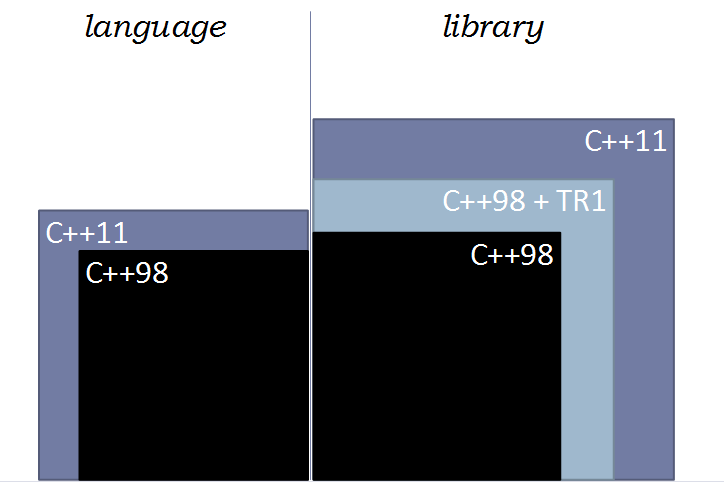
\includegraphics[height=0.7\paperheight]{cpp_libs}}
            \only<2>{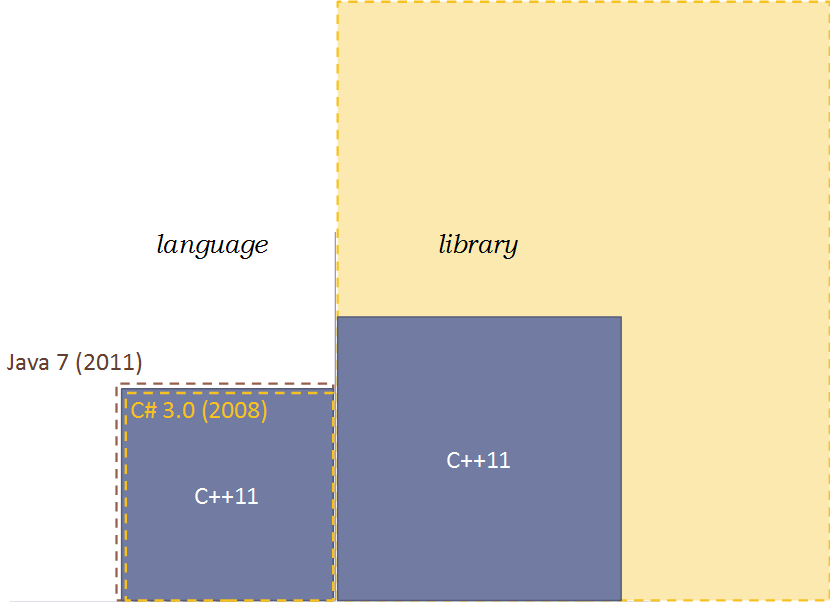
\includegraphics[height=0.85\paperheight]{cpp11_lib}}
            \only<3>{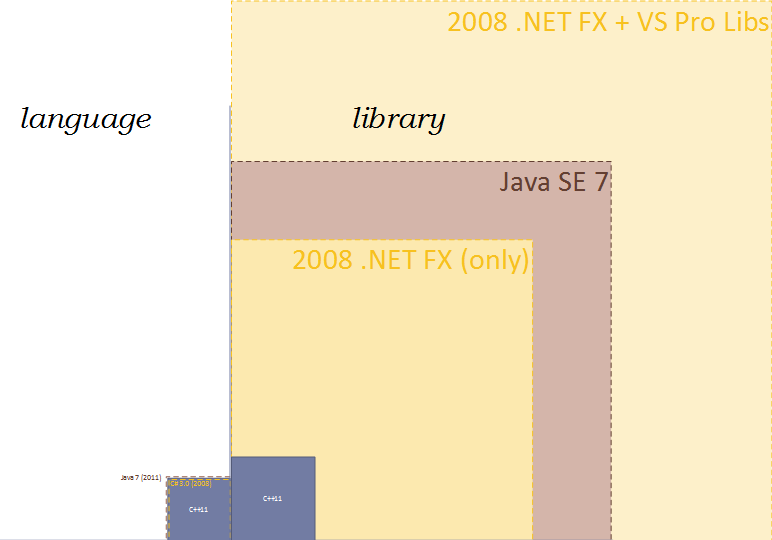
\includegraphics[height=0.8\paperheight]{cpp11_lib2}}\\
            \only<4>{\centering 
\includegraphics[height=0.8\paperheight]{bloated-jabbascript-frameworks}}
        \end{column}
    \end{columns}
}

\section{(R)evolution!}


\slide{(R)evolution!}{
    \centering
    \only<1>{\LARGE Evolution of C++ vs Revolution of C++}
    \only<2>{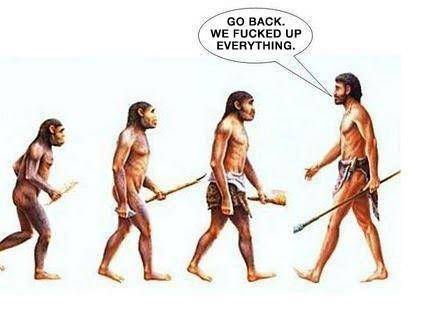
\includegraphics[height=0.8\paperheight]{devolution}}
    \only<3>{
\includegraphics[height=0.8\paperheight]{your-cat-is-evolving}}
}


\slide{C++ is becoming more and more complicated...}{
    \centering
    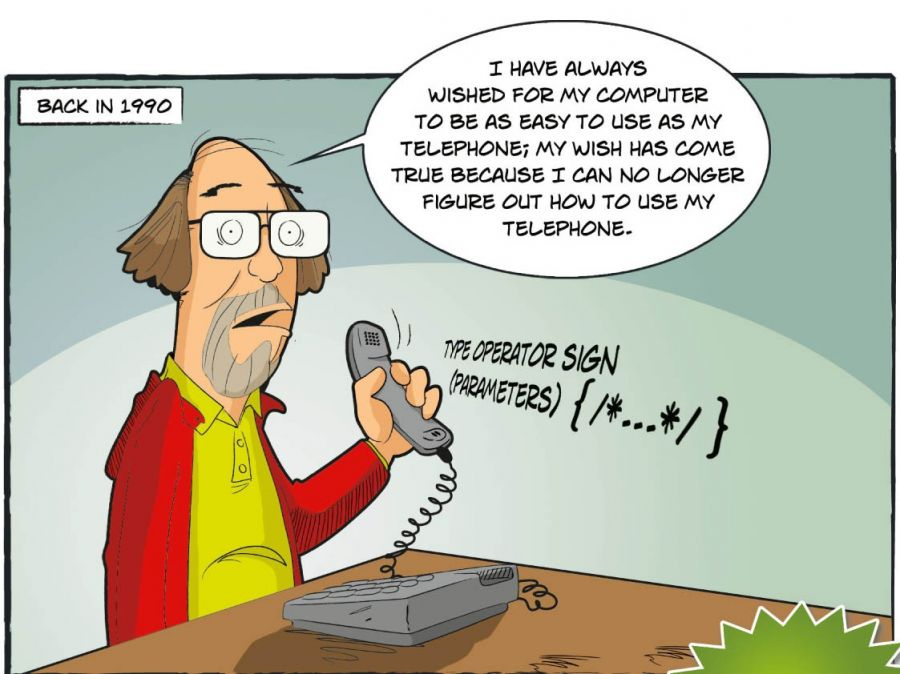
\includegraphics[height=0.8\paperheight]{bjarne-telephone}
}


%TODO: jakiś obrazek plątaniny porównujący skomplikowanie języka kiedyś i dziś
%TODO: jakieś zdjęcie z zarzutami
%TODO: pomyśleć o filmie 
\slide{stdlib is poor}{
    \begin{columns}
        \begin{column}{0.3\textwidth}
            \begin{itemize}[<+->]
                \item Some people say that C++ standard library is small...
                \item In comparison with other languages
                \item Examples from presentation \textit{"One C++"} by Herb Sutter
                \item But it will grow in next standards
            \end{itemize}
        \end{column}
        \begin{column}{0.7\textwidth}
            \only<1>{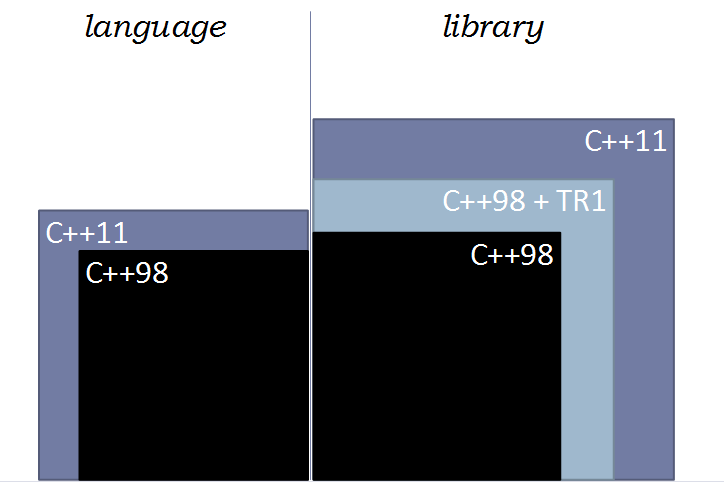
\includegraphics[height=0.7\paperheight]{cpp_libs}}
            \only<2>{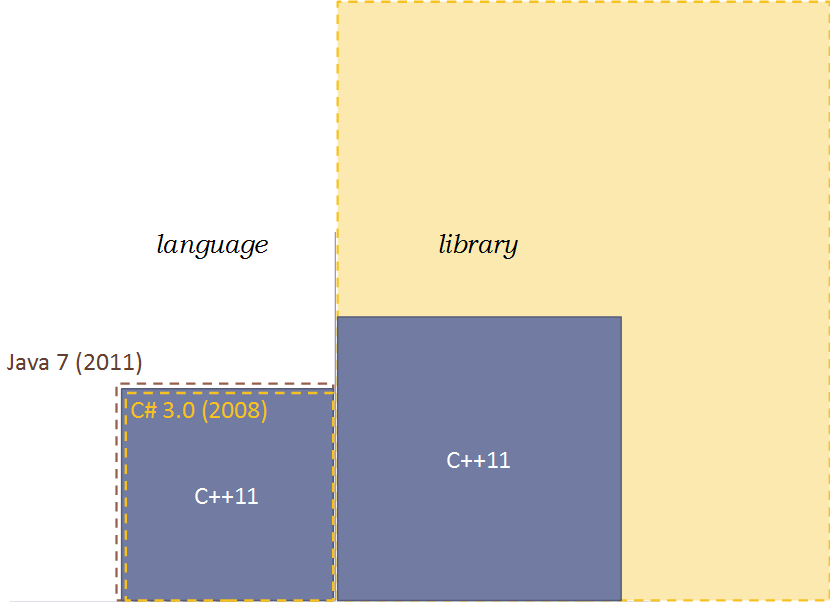
\includegraphics[height=0.85\paperheight]{cpp11_lib}}
            \only<3>{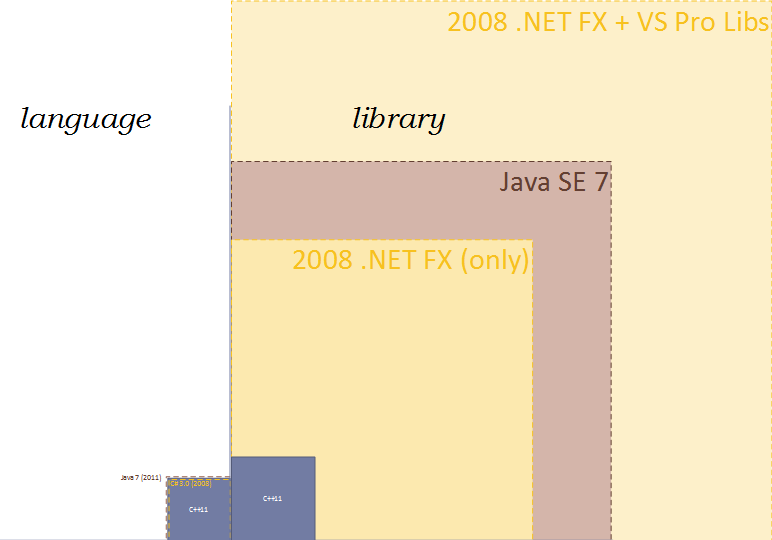
\includegraphics[height=0.8\paperheight]{cpp11_lib2}}\\
            \only<4>{\centering 
\includegraphics[height=0.8\paperheight]{bloated-jabbascript-frameworks}}
        \end{column}
    \end{columns}
}


\slide{C++ standard implementation delays}{
    \begin{table}
        %\caption{C++ users}
        \begin{tabular}{|l|r|r|} %TODO: Wiersz po wierszu niech się pojawia albo zaznaczenie zielonym
            \hline \textbf{Version} & \textbf{Standard} & \textbf{First implementation} \\
            \hline 
            \hline C84 & "the ARM" - 1989 & - \\
            \hline
            \hline C++98 & IX 1998 & 2003 (EDG + Dinkumware) \\
            \hline C++03 & X 2003 & ? \\
            \hline C++11 & IX 2011 & IV 2013 (clang3.3) \\
            \hline C++14 & III 2014 & XI 2013 (clang 3.4) \\
            \hline C++17 & ? & ? \\
            \hline
        \end{tabular}
    \end{table}
}


\slide{Free lunch is over}{
    \begin{columns}
    \begin{column}{0.57\textwidth}
        \begin{itemize}[<+->]
            \item Moore's law is no applicable anymore % Free lunch is over
            \item Processor speed doesn't rise
            \item We must go into concurrency
            \item We must write multithreaded apps
            \item We must write efficient and effective code
            \item Modern C++ facilitate above needs % Effective modern C++
            \item VM languages will not be faster than C++
            \item More and more mobile apps are written in C++
            \item Can C perform better? %TODO: QR kod do prezentacji Bartosza
        \end{itemize}
    \end{column}
    \begin{column}{0.43\textwidth}
        \only<1-5>{\centering 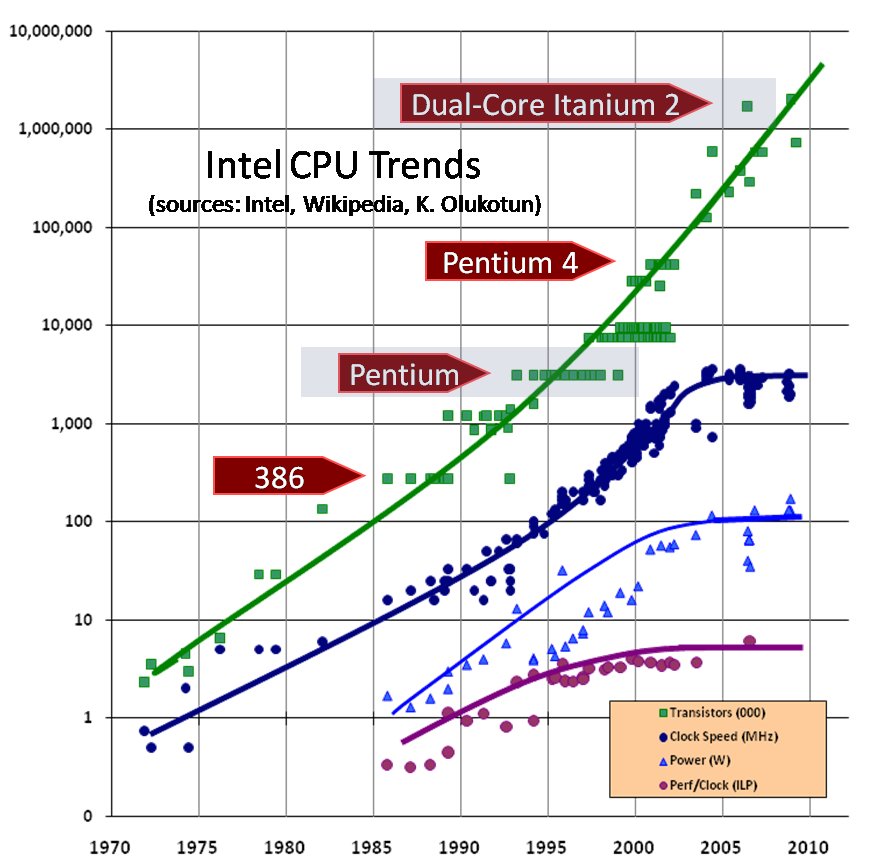
\includegraphics[height=0.6\paperheight]{free-lunch-is-over} \\
                   \scriptsize \url{http://www.gotw.ca/publications/concurrency-ddj.htm}}
        \only<6-8>{\centering 
\includegraphics[height=0.7\paperheight]{effective-modern-cpp} \\
                   \scriptsize (This book cover is real)}
        \only<9>{\centering 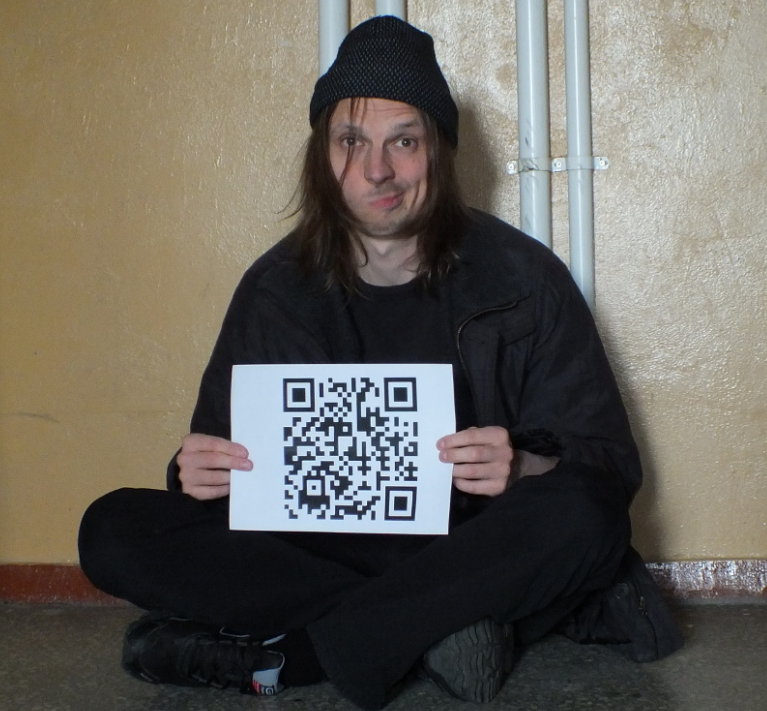
\includegraphics[height=0.6\paperheight]{szurgot} \\
                {\scriptsize Bartosz 'BaSz' Szurgot \\ C++ vs. C: The embedded perspective \\ code::dive 2015 }}
    \end{column}        
    \end{columns}
}
\sectionSlide{Language popularity}{languages-popularity}{\paperwidth}{t}

\slide{What is the most popular programming language?}{
    \centering
    
\includegraphics[height=0.8\paperheight]{it-depends}
}

\slide{C++ users}{
    \begin{columns}
        \begin{column}{0.5\textwidth}
            {\small 
                \begin{table}
                    %\caption{C++ users}
                    \begin{tabular}{|l|r|}
                        \hline \textbf{Date} & \textbf{Estimated users} \\
                        \hline 
                        \hline 1979 & 1 \\
                        \hline 1980 & 16 \\
                        \hline 1981 & 38 \\
                        \hline 1982 & 85 \\
                        \hline 1983 & ??+2 \\
                        \hline 1984 & ??+50 \\
                        \hline 1985 & 500 \\
                        \hline 1986 & 2 000 \\
                        \hline 1987 & 4 000 \\
                        \hline 1988 & 15 000 \\
                        \hline 1989 & 50 000 \\
                        \hline 1990 & 150 000 \\
                        \hline 1991 & 400 000 \\
                        \hline
                    \end{tabular}
            \end{table}}        
        \end{column}
        \begin{column}{0.5\textwidth}
            \pause
            Main users:
            \itemstep{
                \item Bjarne,
                \item Bjarne's colleagues from AT\&T Bell Labs,
                \item universities,
                \item HP, IBM, AT\&T, DEC,
                \item Borland,
                \item Later: Microsoft, Apple,
                \item Now: Google, Facebook
            }
        \end{column}
    \end{columns}
}


\slide{C++ users}{
    \centering 
    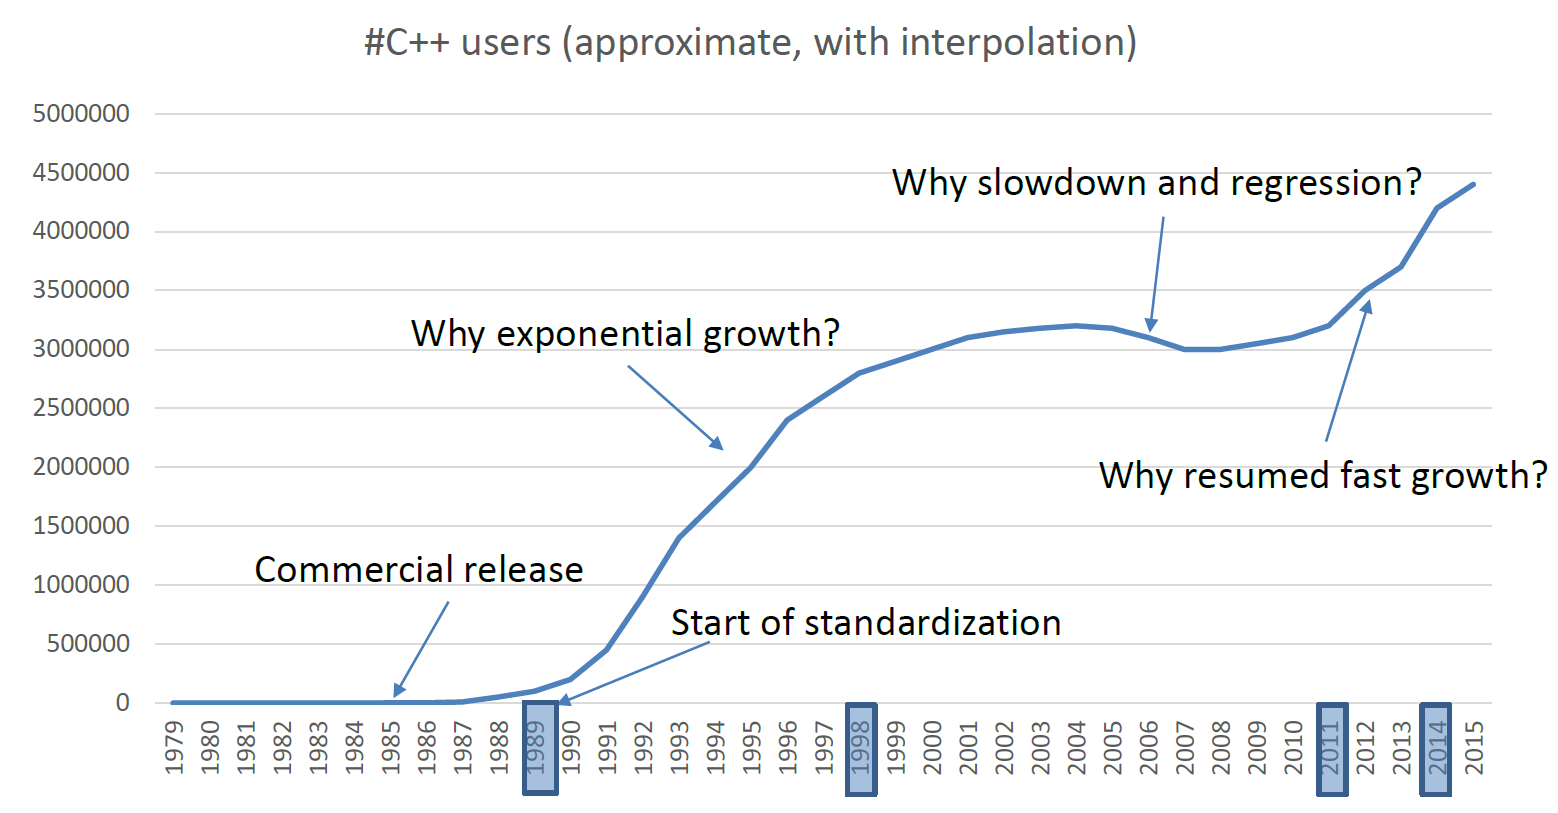
\includegraphics[height=0.8\paperheight]{cpp_users} %TODO: Loga firm na wykresie dodać
    %TODO: wyrzucić pytania, zostawić hasła
}


\slide{TIOBE - market share}{
    \only<1>{
        \begin{block}{TIOBE index}
            \textbf{The TIOBE Programming Community} index is an indicator of the popularity of programming languages. The index is updated once a month. Popular search engines such as \textbf{Google, Bing, Yahoo!, Wikipedia, Amazon, YouTube} and \textbf{Baidu} are used to calculate the ratings. Search phrase is \textbf{"language programming"} \\
            Webpage: \url{http://www.tiobe.com/tiobe-index//}
        \end{block}
    }
    \centering 
    \includegraphics<2>[height=0.7\paperheight]{tiobe-graph-grey}
    %TODO: Na dole zielona krecha C++
    \includegraphics<3>[height=0.7\paperheight]{tiobe-graph}
    \includegraphics<4>[height=0.7\paperheight]{tiobe-array} % TODO: zaznaczyć gdzie jest C++  
}


\slide{PYPL}{
    \only<1>{
        \begin{block}{PYPL index}
            \textbf{The PYPL PopularitY of Programming Language} Index is created by analyzing how often \textbf{language tutorials} are searched on Google: the more a language tutorial is searched, the more popular the language is assumed to be. It is a leading indicator. The raw data comes from \textbf{Google Trends}. \\
            Webpage: \url{http://pypl.github.io/PYPL.html}  
        \end{block}
    }
    \centering 
    \includegraphics<2>[height=0.8\paperheight]{pypl-graph-grey}
    %TODO: Lepiej opisać wykres
    \includegraphics<3>[height=0.8\paperheight]{pypl-graph}
    \includegraphics<4>[height=0.8\paperheight]{pypl-array}
}


\slide{codeeval}{
    \only<1>{
        \begin{block}{codeeval MPCL}
            \textbf{"Most Popular Coding Languages"} is based on hundreds of thousands of data points we've collected by processing over 1,200,000+ \textbf{challenge submissions on codeeval.com} in (now) 26 different programming languages. \\
            Webpage: \url{http://blog.codeeval.com/}  
        \end{block}
    }
    \centering 
    \includegraphics<2>[height=0.83\paperheight]{codeeval2016}
    \includegraphics<3>[height=0.83\paperheight]{codeeval2015}
%    \includegraphics<4>[height=0.34\paperheight]{codeeval2014}
}


\slide{langpop.corger.nl}{
    \centering
    
\includegraphics[height=0.5\paperheight]{github-logo} \vline
    
\includegraphics[height=0.5\paperheight]{stackoverflow-logo} \\
    Webpage: \url{http://langpop.corger.nl/} 
}


\imageSlide{langpop-graph} %TODO: Lepiej oznaczyć osie


\slide{Stackoverflow issues}{
    \begin{columns}
    \begin{column}{0.6\textwidth}
        \itemstep{
            \item good programmer == lazy programmer
            \item lazy programmer != good programmer
            \item good programmers do not reinvent the wheel
            \item do job once and never come back here
        }
    \end{column}
    \begin{column}{0.4\textwidth}
        \centering 
        \includegraphics<3->[height=0.8\paperheight]{copying-and-pasting-from-stack-overflow}
    \end{column}
    \end{columns}
}


\slide{C++ is not dead!}{
    \begin{columns}
    \begin{column}{0.6\textwidth}
        \begin{itemize}
            \item In the worst case C++ is on 7th place
            \item In the best case C++ is on 3rd place
            \item C++ is one of the most popular languages!
    		\item There will be next versions of C++ %TODO: przeredagować jeszcze
        \end{itemize}
    \end{column}
    \begin{column}{0.4\textwidth}
        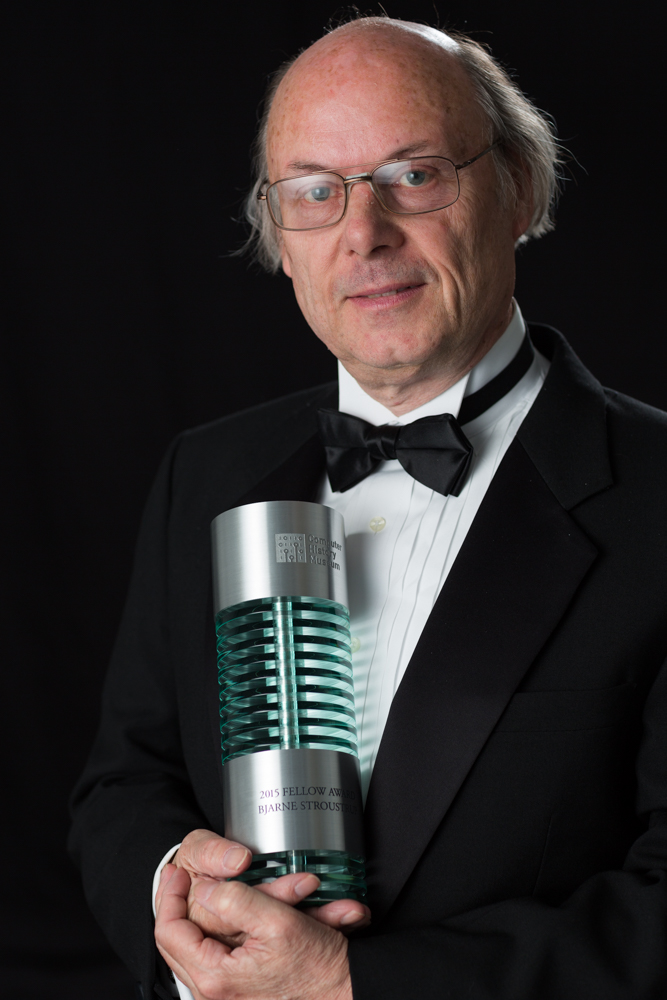
\includegraphics[height=0.8\paperheight]{bjarne-stroustrup}
    \end{column}
    \end{columns}
}
\sectionSlide{Summary}{c++-logo}{0.9\paperheight}{b}


\slide{Key messages}{
    \Large 
    \enumstep{
        \item C++ had a clear aim, which made it popular: to organize code better without the loss of efficiency
        \item C++ is even more popular now, because of new standards: C++11 and C++14.
        \item C++ will be one of the most popular programming languages in future so it's worth to invest in learning it.
    }
}


\slide{Worth reading / watching}{
    \begin{thebibliography}{9}
        \setbeamertemplate{bibliography item}[online]
        \bibitem{Stroustrup} Bjarne Stroustrup -- \textit{The Evolution of C++ - Past, Present, and Future} \\
        {\scriptsize CppCon 2016 \\ \url{https://www.youtube.com/watch?v=_wzc7a3McOs}}
        \bibitem{Sutter} Herb Sutter -- \textit{One C++} \\
        {\scriptsize Going Native 2013 \\ \url{https://channel9.msdn.com/Events/GoingNative/2013/Keynote-Herb-Sutter-One-Cpp}} 
        \bibitem{Gregory} Kate Gregory -- \textit{Stop teaching C} \\
        {\scriptsize CppCon 2015 \\ \url{https://www.youtube.com/watch?v=YnWhqhNdYyk}}    
        \setbeamertemplate{bibliography item}[article]
        \bibitem{Stroustrup2} Bjarne Stroustrup -- \textit{A History of C++: 1979-1991} \\
        {\scriptsize \url{http://www.stroustrup.com/hopl2.pdf}}
        \setbeamertemplate{bibliography item}[book]
        \bibitem{Meyers} Scott Meyers -- \textit{Effective Modern C++}
    \end{thebibliography}
}


\slide{What's now?}{
    \begin{block}{What's now?}
        \itemstep{
            \item Look forward to C++17 and learn it
            \item Watch a lot of videos from C++ conferences
            \item Visit \url{isocpp.org}
        }
    \end{block}

    \pause
    \begin{block}{}
        \begin{quotation}
            {\Large ``Learn C++. It's an investment.''}
        \end{quotation}
        \pause
        \rightline{{\rm --- Łukasz Ziobroń}}
	%TODO: nowy slajd + zdjęcie coachingowe
    \end{block}
}


\imageSlide{keep-calm-and-ask-questions}


